\documentclass{report}

\usepackage[pdftex]{graphicx}
\usepackage{parskip}


\begin{document}
\title{1200 baud AFSK Demodulation: A cheap solution to hardware TNCs}
\author{Robert Campbell}
\maketitle

\begin{abstract}
In amateur radio APRS had evolved, but it like many other things in the
amateur radio community continues to lag behind current times, not taking
full advantage of new technologies. The goal here is to introduce a new
software suite that makes the decoding of APRS packets more reliable and
at a cheap price. Having hardware TNCs can be a very expensive barrier to
entry, but already having a computer is pretty common these days.
\end{abstract}

\tableofcontents

\chapter{Introduction}

Amateur Radio Operators, commonly referred to as "hams," make the best of resources available to them. However, once something is working a "don't touch it if it ain't broke" approach is often taken. Between these two mentalities some interesting phenomenon have occurred within the ham community. For example, some radio systems that are in active service today have only seen very minimal attention since the 1980's when they were originally installed. The implementation and development of the Automated Packet Reporting System (APRS) is no exception to the way hams approach things\,\cite{Bruninga}. Much of this system is based off older hardware and protocols - from the 1980s - that was readily available and few improvements have been made. Unfortunately, although the specification has been relatively stable there are inconsistencies. These inconsistencies include varying implementations from vendor to vendor as well as portions of the specification that are not clearly defined resulting in vastly inconsistent performance\,\cite{KWFThesis, KWFTAPR}.

So, what is APRS, and why does it matter? A brief introduction to APRS is that it is a digital communication scheme used by hams where a packet (whose content is varied, but is usually a GPS position - which is what gave APRS it's original name "Automated Position Reporting System"\cite{WikiAPRS}) is sent out over radio and then interpreted by other receiving stations. Figure \ref{APRSEndToEnd} shows one example of an end to end APRS system. A major challenge to this protocol and many other method of digital communication is the fact that it uses radio. Transmitting the signal wirelessly over radio means that it is susceptible to interference, weak signals as the distance from the transmitting station increases, as well as a myriad of other items. This research focuses specifically on the receiving end of these signals in order to see what improvements can be made to software based approaches to demodulating (decoding) these packets, which is represented by the TNC block in Figure \ref{APRSEndToEnd}. However, to more accurately portray software based demodulation the TNC block in the figure should be moved inside of the computer block since the receive radio audio is passed straight to the computer and then interpreted by this special software.

\begin{figure}
  \centering
	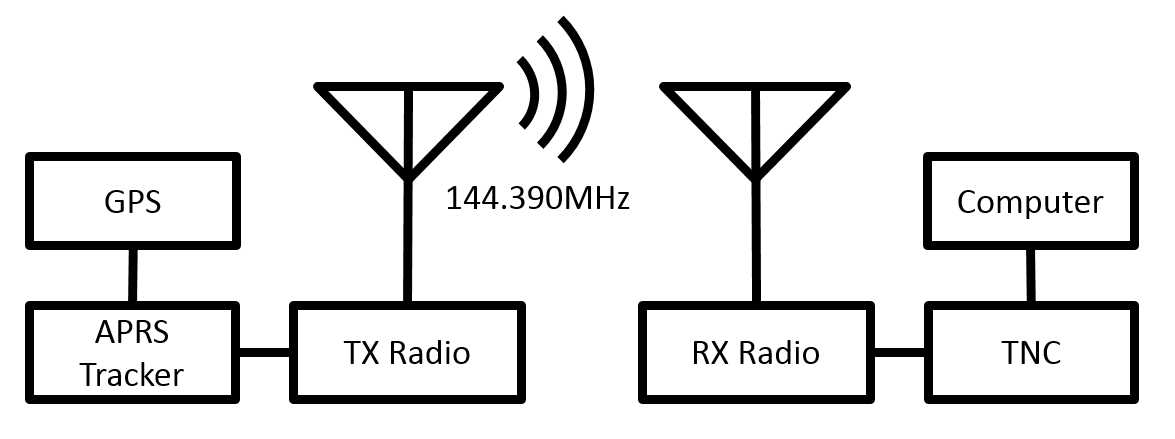
\includegraphics[width=0.75\linewidth]{images/APRSEndToEnd.PNG} 
   \caption[Block diagram of an example APRS system end to end.]{Block diagram of an example APRS system end to end. The GPS communicates information using NEMA to the APRS tracker, the tracker then takes this information and the preferences in its configuration to formulate APRS packets. The APRS packets are encoded by the tracker and the resulting audio passed to a transmit radio which sends the data. Typically this is done on frequency 144.390MHz in the United States. Receiving radios tuned to the same frequency pass the received audio to a TNC which decodes the packet and passes it to a computer using RS-232.}
   \label{APRSEndToEnd}
\end{figure}

The reasoning for trying to make improvements in software based demodulation are many, but a few of the more motivational ones are to follow. One advantage of doing software based demodulation is that it removes the necessity of specialty hardware; Instead of having dedicated hardware whose sole purpose is to modulate and demodulate APRS packets, hams can use a computer to do these tasks. By using a computer's sound card, audio from the radio can be processed using software to decode received packets, or audio can be played from the sound card to the radio to be transmitted. With the abundance of personal computers, this can provide a much cheaper solution for hams who are interested in trying out APRS without having to put down a potentially big initial investment (\textasciitilde\$200\,\cite{Kantronics2014,Outlet2014}) for a piece of hardware that serves one purpose. The price of this specialty hardware is steep and it is limited to only performing communication on a single channel. When using a line in / out on a computer they are typically stereo, meaning that a single sound card could handle operations on multiple channels. If two channels just is not enough the capabilities of a computer demodulator can be expanded by merely adding another sound card which is relatively cheap at \textasciitilde\$20\,\cite{Newegg}. See Table \ref{costCompareTable} for a comparison of the cost for hardware and software. From the table it can be seen that the cost to perform communication on 4 channels using dedicated hardware the cost would be \$800! For this cost a whole computer with a half dozen sound cards could be purchased, only further expanding capabilities.

\begin{table}
	\begin{center}
		\begin{tabular}{ | l | r | r | r | r | }
		\hline
			Cost for: & 1 Channel & 2 Channels & 3 Channels & 4 Channels \\ \hline
			Software & \$0 & \$0 & \$20 & \$20 \\ \hline
			Hardware & \$200 & \$400 & \$600 & \$800 \\
			\hline
		\end{tabular}
		\caption[Hardware and Software Cost Comparison]{Cost comparison of conducting APRS communications on 1 through 4 channels for hardware versus software assuming the user already owns a computer.}
		\label{costCompareTable}
	\end{center}
\end{table}

In addition to the the price advantages of software based demodulation approaches, there is also one other primary advantage. If software is being used instead of hardware there is the potential for a lot more capabilities since processing power and available memory increase drastically. For instance, one of the dedicated hardware solutions, the Kantronics KPC-3 Plus, has a mere 512KB of memory compared to that of any computer which is over 4GB as of 2014 - and that is just the ram, not hard drive space\,\cite{Kantronics2014,Graham-Smith2014}. Additionally, instead of just being able to handle live events and process each data point in the best manner possible as soon as it comes in, post processing becomes an option.

With the cost and versatility of a software demodulation solution now introduced, the paper addresses the following: Chapter 2 goes into background information, with a deeper introduction to APRS and a presentation of the aspects important to understanding this research. In Chapter 3, some of the current methods for interfacing with APRS, both hardware and software, are explained. Demodulation techniques are discussed in Chapter 4. Chapter 5 talks about the challenges of demodulating APRS packets. Chapter 6 discusses the methods used for benchmarking and comparing the demodulators. In Chapter 7, information on how the demodulators and algorithms are tested is presented. Chapter 8 goes into more detail about the software implementations in this project. Chapter 9 discusses the results of both the newly implemented algorithms and compares them to other demodulators. Areas of additional research and future work are discussed in Chapter 10. Chapter 11 is concluding remarks.


\end{document}
